% \pdfminorversion=4
\documentclass{beamer}
\usepackage[utf8]{inputenc}
\usepackage{indentfirst}
\usepackage{enumitem}
\usepackage{datetime2}
\usepackage{acronym}
% options (https://tex.stackexchange.com/questions/25520/how-can-i-use-the-latex-acronym-package-and-optionally-create-an-acronym-list-i):
% printonlyused: Only list used acronyms
% withpage: In printonlyused-mode show the page number where each acronym was first used.
% nolist: The option nolist stands for “don’t write the list of acronyms”.
% dua: The option dua stands for “don’t use acronyms”. It leads to a redefinition of \ac and \acp, making the full name appear all the time and suppressing all acronyms but the explicity requested by \acf or \acfp.

\makeatletter
\AtBeginDocument{%
  \renewcommand*{\AC@hyperlink}[2]{%
    \begingroup
      \hypersetup{hidelinks}%
      \hyperlink{#1}{#2}%
    \endgroup
  }%
}
\makeatother

\usepackage{algorithm}
\usepackage{algpseudocode}

\usepackage{textcomp}
\usepackage[T1]{fontenc}
\usepackage{multirow,bigdelim}
\usepackage{float}
\usepackage[caption = false]{subfig}
\usepackage{longtable}
\usepackage{listings}
\usepackage{mathtools}
\DeclareMathOperator{\tr}{Tr}
\usepackage{commath}
\usepackage{slashed}
\usepackage{bbold}
\usepackage{xcolor}
\usepackage{physics}
\newcommand{\lambdabar}{{\mkern0.75mu\mathchar '26\mkern -9.75mu\lambda}}
\usepackage[right=4cm,left=2cm,top=3cm,bottom=3.0cm, marginparwidth=2.7cm, marginparsep=3mm]{geometry}
\usepackage{mdframed}


\usepackage{amsmath}
\usepackage{amsfonts}
\usepackage{amssymb}

\numberwithin{equation}{section}
\usepackage{graphicx}

\usepackage[colorinlistoftodos]{todonotes}
\PassOptionsToPackage{hyphens}{url}
\usepackage[colorlinks=true, allcolors=blue]{hyperref}
\hypersetup{breaklinks=true}

% \urlstyle{same}
\usepackage{siunitx}
\sisetup{separate-uncertainty=true}
% \DeclareSIUnit\parsec{pc}
\usepackage{cancel}
\usepackage{mathrsfs}
\usepackage{marginnote}
\renewcommand*{\marginnotevadjust}{-0.3cm}
\renewcommand*{\marginfont}{\scriptsize}
% \usepackage{fancybox}

\usepackage{footnotebackref}

\usepackage[sc]{mathpazo}
\linespread{1.05}         % Palladio needs more leading (space between lines)
\usepackage[T1]{fontenc}

\newcommand\mybox[1]{%
  \fbox{\begin{minipage}{0.9\textwidth}#1\end{minipage}}}

\newcommand{\const}{\mathrm{const}}

\usepackage[section]{placeins}

\usepackage{tikz}
\usetikzlibrary{shapes,arrows,shadows}


\newcommand{\boxalign}[2][0.986\textwidth]{
  \par\noindent\tikzstyle{mybox} = [draw=black,inner sep=6pt]
  \begin{center}\begin{tikzpicture}
   \node [mybox] (box){%
    \begin{minipage}{#1}{\vspace{-5mm}#2}\end{minipage}
   };
\end{tikzpicture}\end{center}}


\pagestyle{plain}

\author{Jacopo Tissino}

\allowdisplaybreaks
\usetheme{Rochester}
% \usepackage[scaled]{helvet} % ss

\usepackage[
backend=biber,
style=authoryear,
sorting=nyt,
urldate=iso8601,
url=false,
isbn=false,
doi=false
]{biblatex}

\title{Machine Learning Gravitational Waveforms for Binary Neutron Star mergers}
\author{Jacopo Tissino}
\date{2021-07-28}

\addbibresource{../notes/Masters_thesis.bib}


\begin{document}

\frame{\titlepage}

\begin{frame}
    \frametitle{GW170817: the first BNS merger detection}
    \begin{columns}
        
    \begin{column}{0.5\textwidth}
    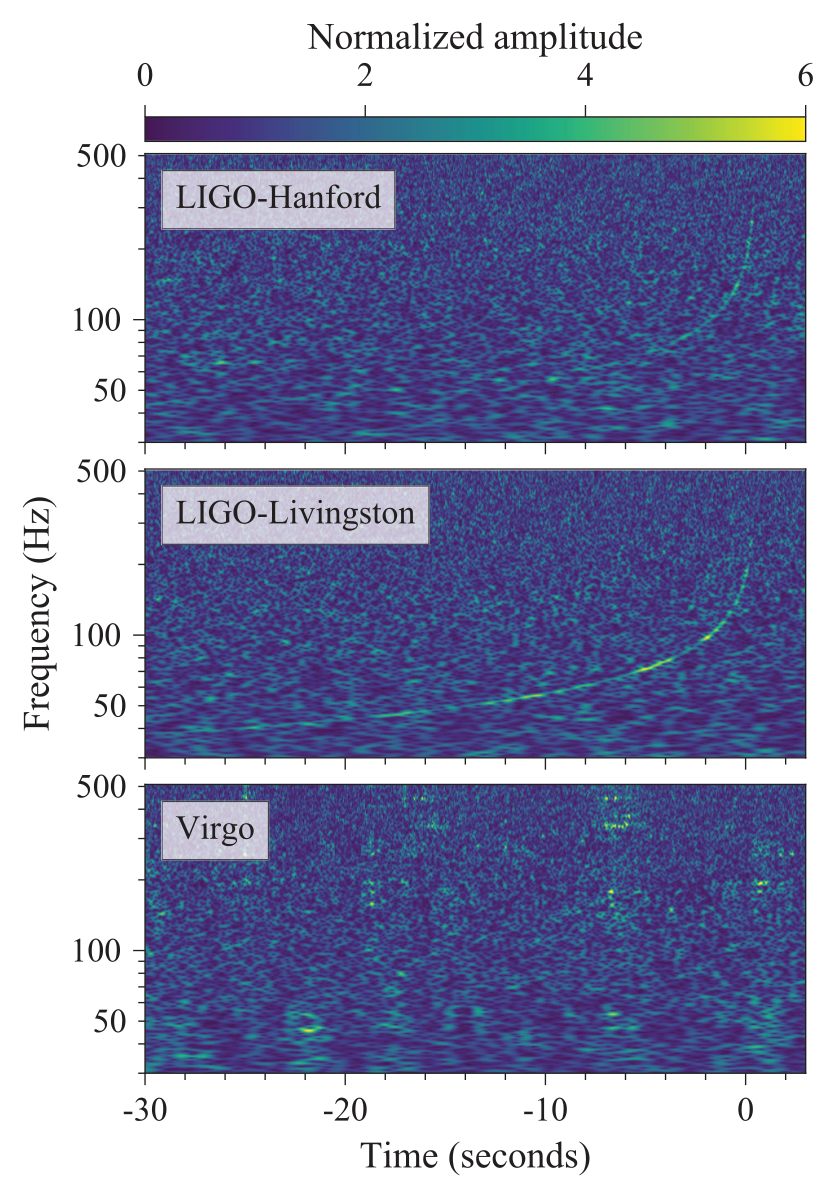
\includegraphics[width=\textwidth]{figures/836px-GW170817_spectrograms.svg.png}
    \end{column}

    \begin{column}{0.5\textwidth}
    Time-frequency representation of the chirping waveform
    (\cite[]{abbottGW170817ObservationGravitational2017}).

    BNS waveforms are much longer than BBH ones: they only depend on \(t/M \) (or \(fM\)), where \(M = m_1 + m_2 \) is the total mass.
    \end{column}
    \end{columns}
\end{frame}

\begin{frame}
    \frametitle{GW data analysis}
    
    \begin{itemize}
        \item Signal from detector: \(s(t) = h(t) + n(t)\), with noise PSD \(S_n (f)\);
        \item Theoretical waveforms \(h_\theta (t)\):
        \begin{itemize}
            \item Numerical Relativity;
            \item Effective One Body;
            \item Post-Newtonian;
        \end{itemize}
        \item Signal searches;
        \item Parameter estimation and model comparison.
    \end{itemize}

The parameters \(\theta \) are divided into 
\begin{itemize}
    \item intrinsic ones: masses \(m_i\), spins \(\vec{\chi}_i\), tidal deformabilities \(\Lambda_i\);
    \item extrinsic ones: luminosity distance \(D_L\), source inclination \(\iota \), sky position \((\alpha , \delta )\), polarization angle \(\psi \), reference time \(t_0 \) and phase \(\phi_0 \).
\end{itemize}
\end{frame}

\begin{frame}
    \frametitle{The Wiener distance}
    
    The likelihood used in parameter estimation reads (\cite[]{maggioreGravitationalWavesVolume2007}): 
    %
    \begin{align}
    \Lambda (s | \theta ) \propto \exp( (h_\theta | s) - \frac{1}{2} (h_\theta | h_\theta ))
    \,,
    \end{align}
    %
    where \((a | b)\) is the Wiener product: 
    %
    \begin{align}
    (a | b) = 4 \Re \int_{0}^{\infty } \frac{\widetilde{a}^{*}(f) \widetilde{b} (f)}{S_n (f)} \dd{f}
    \,.
    \end{align}
    
    We need a fast way to compute accurate theoretical waveforms \(h_\theta \) in the frequency domain! Typical EOB evaluation times are \(\sim \SI{100}{ms}\) for \(f_0 = \SI{20}{Hz}\), \(\sim \SI{1}{s}\) for \(f_0 = \SI{10}{Hz}\). 
\end{frame}

\begin{frame}
    \frametitle{Frequency domain waveforms: amplitude}

    \centering
    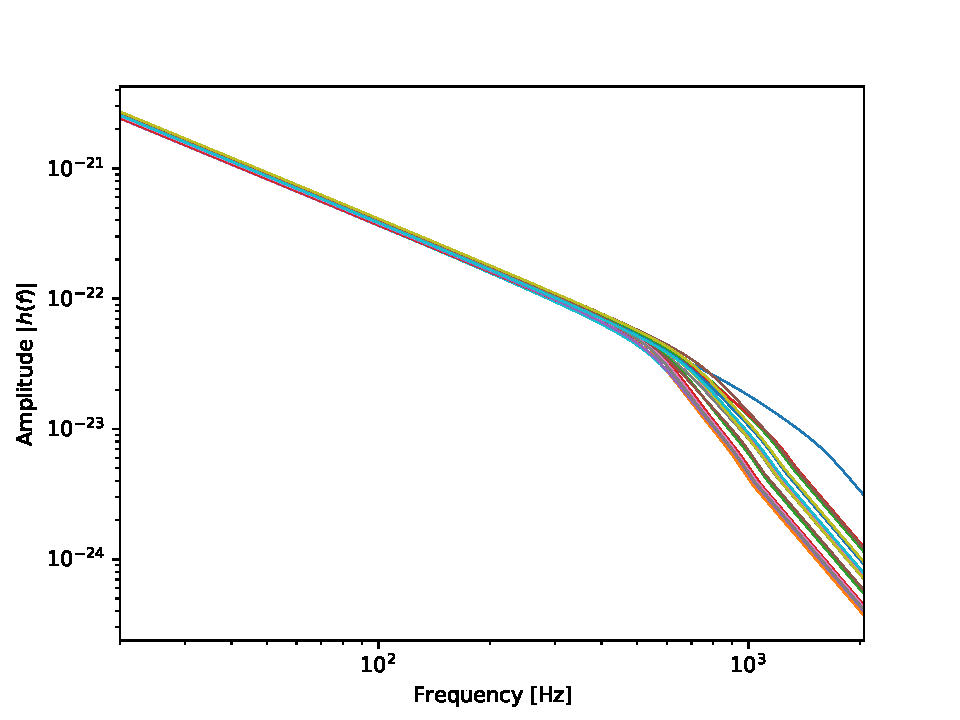
\includegraphics[width=.9\textwidth]{figures/amplitude_random.pdf}
\end{frame}

\begin{frame}
    \frametitle{Frequency domain waveforms: phase}

    \centering
    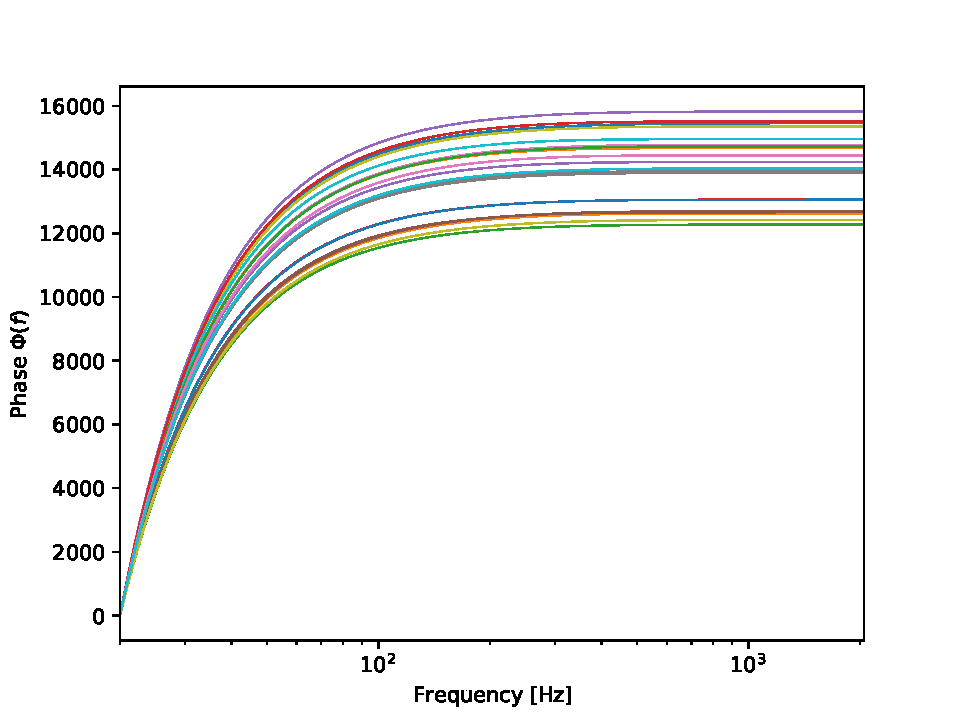
\includegraphics[width=.9\textwidth]{figures/phase_random_semilog.pdf}
\end{frame}

\begin{frame}
    \frametitle{\texttt{MLGW\_BNS}}
    
    A fast generator of frequency-domain waveforms, currently varying the mass ratio \(q\) and the tidal deformabilities \(\Lambda_1 \), \(\Lambda_2 \).
    
    \begin{itemize}
        \item A training dataset is generated: residuals of Effective One Body waveforms from the corresponding Post-Newtonian ones;
        \item dimensionality is reduced through Principal Component Analysis;
        \item a feed-forward Neural Network learns the map from the parameters to the principal components: \(\theta \to \qty{\text{PC}_i}_i\).
    \end{itemize}
    
    Reconstruction accuracy is evaluated through a distance induced by the Wiener product: 
    %
    \begin{align}
    \mathcal{F}[a, b] = 1 - \max_{t_0 , \phi_0 } \frac{(a|b)}{\sqrt{(a|a)(b|b)}}
    \,.
    \end{align}

\end{frame}

\begin{frame}
    \frametitle{Reconstruction with PCA}
    
    \centering
    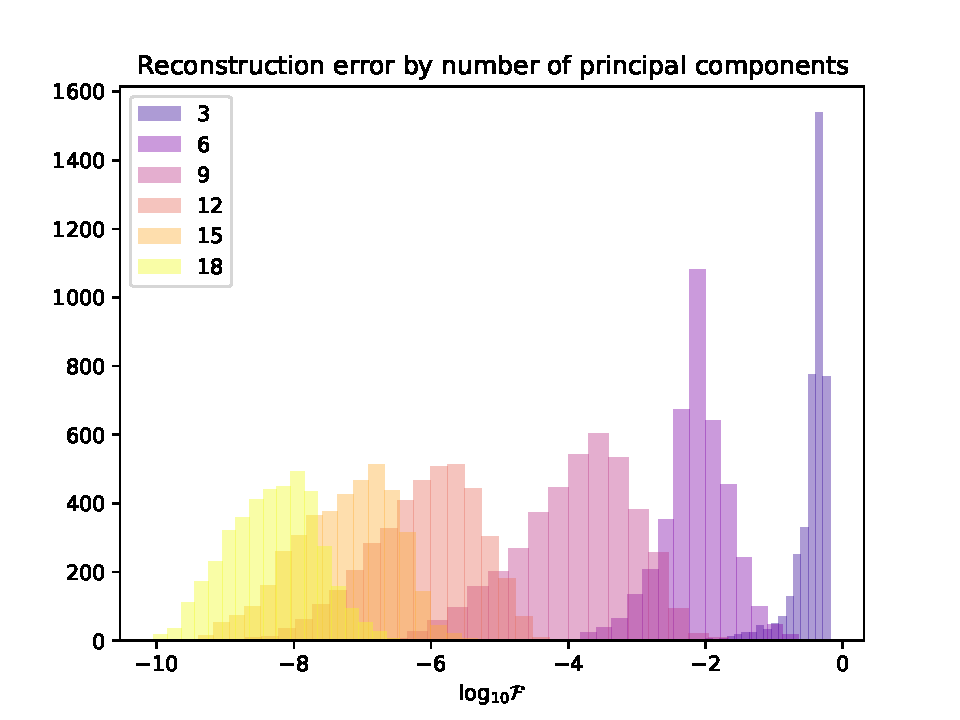
\includegraphics[width=.9\textwidth]{figures/reconstruction_errors_PCA.pdf}
\end{frame}

\begin{frame}
    \frametitle{Reconstruction with \texttt{MLGW\_BNS}: mismatches}
    
    \centering
    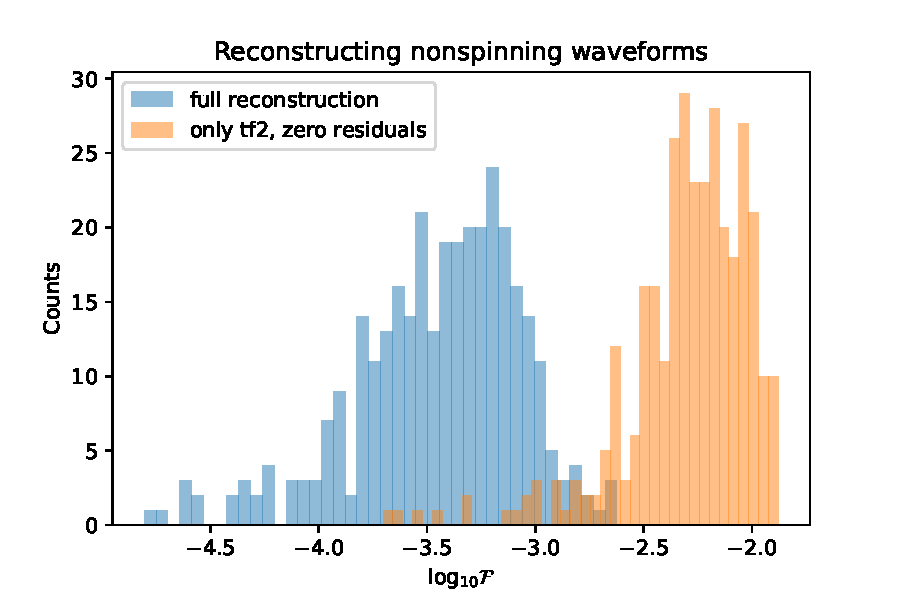
\includegraphics[width=.95\textwidth]{figures/three_param_residuals.pdf}
\end{frame}

\begin{frame}
    \frametitle{Reconstruction with \texttt{MLGW\_BNS}: time domain}
    
    \centering
    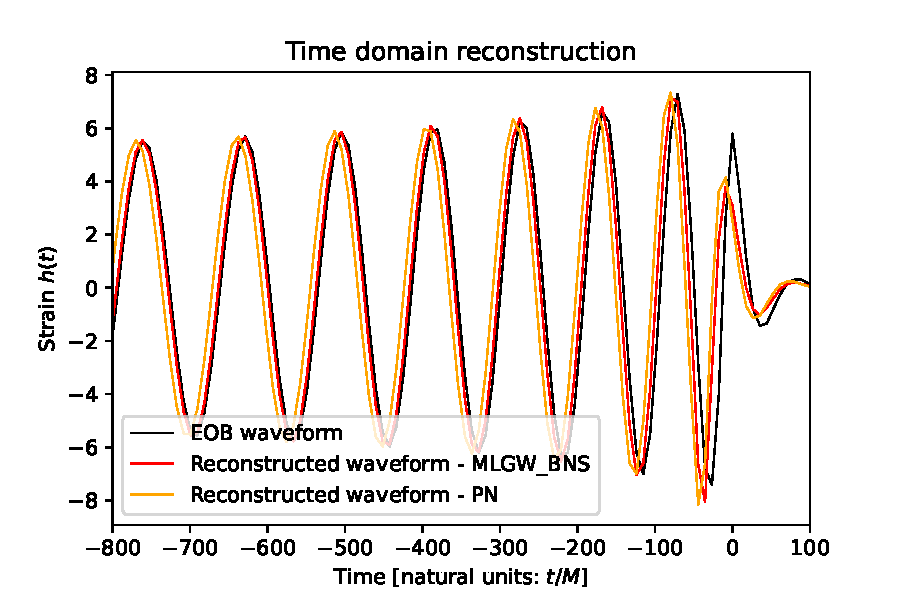
\includegraphics[width=.95\textwidth]{figures/td_comparison.pdf}
\end{frame}

\begin{frame}
    \frametitle{Technologies}
    
    \begin{itemize}
	\item Python wrapper for \texttt{TEOBResumS} for EOB waveform generation;
	\item \texttt{python} with standard scientific libraries (\texttt{numpy}, \texttt{scipy}, \texttt{matplotlib}) and \texttt{pycbc};
	\item Neural Network implemented with \texttt{scikit-learn}, hyperparameters optimized with \texttt{optuna};
	\item automated testing with \texttt{pytest} and \texttt{hypothesis}.
    \end{itemize}
\end{frame}

\begin{frame}
    \frametitle{Bibliography}
    
    \printbibliography
\end{frame}


\end{document}
